\section{Funzionalità dell'applicazione  Android}
\label{sec:sec_funzionalita_applicazione}
\subsubsection{Registrazione}
\label{sec:funzionalita_applicazione_registrazione}
All'interno della applicazione viene data all'utente la possibilità di creare un proprio account, questo è necessario per l'utilizzo dell'applicazione. Per accedere al form di registrazione cliccare su "\textit{Create New Account}":
\begin{figure}[H]
	\centering
	%	\vspace*{-8cm}
	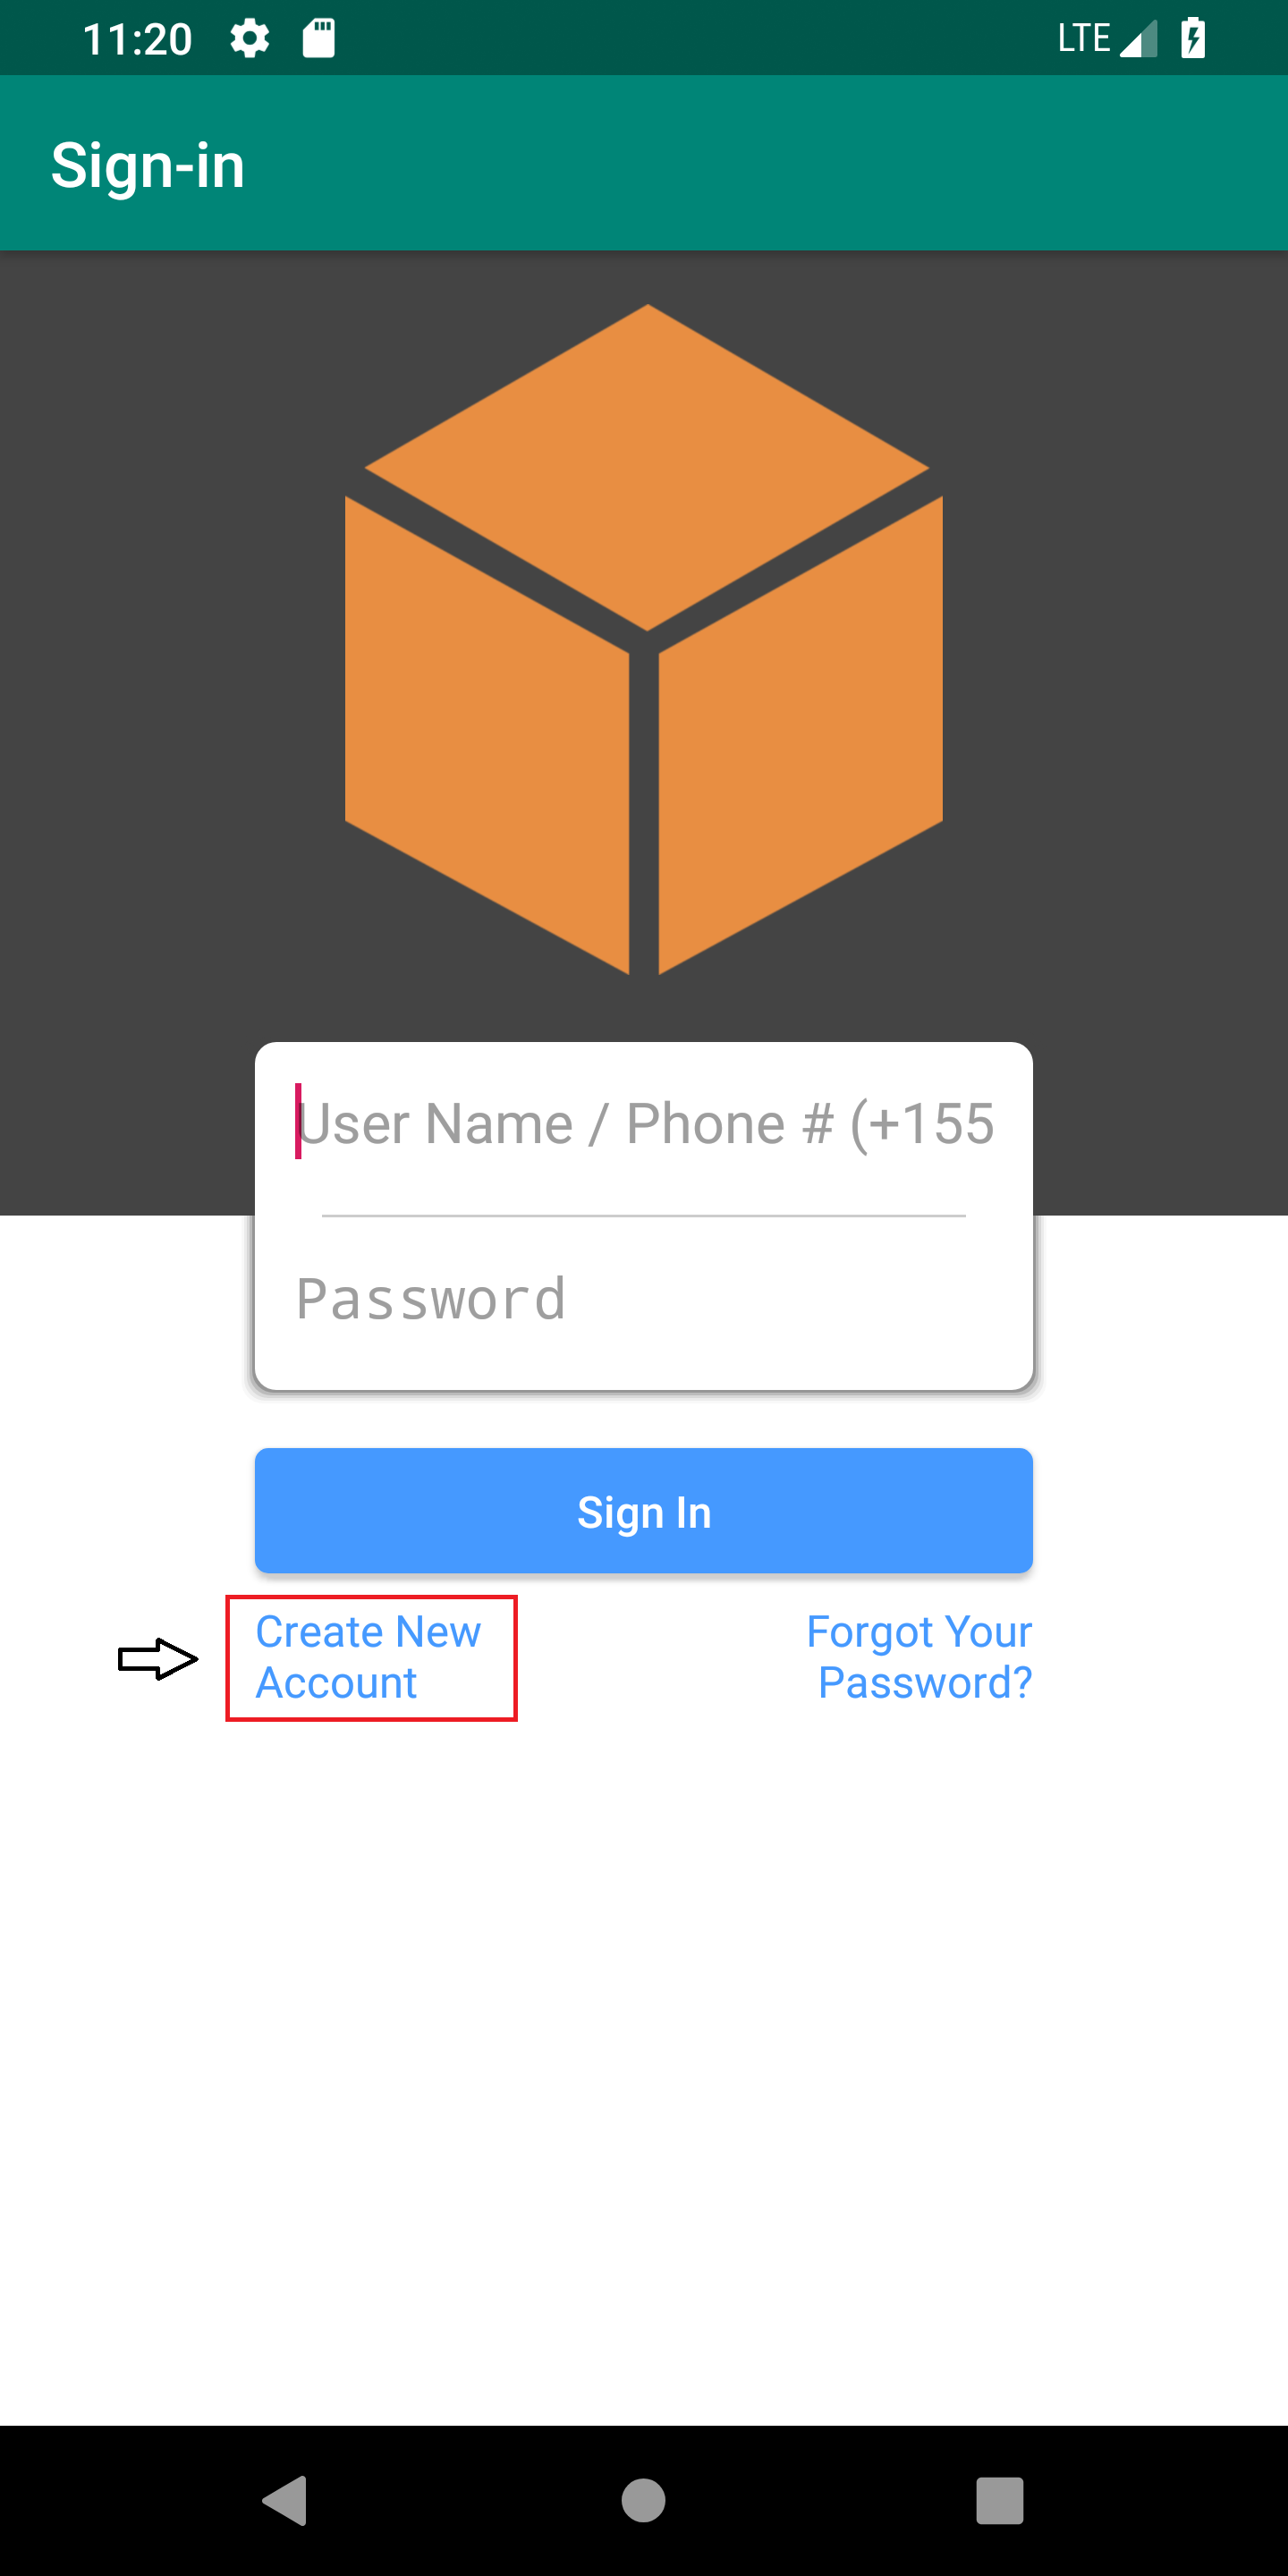
\includegraphics[width=5cm]{../includes/pics/app_registration_form_1.png}
	\caption{\label{fig:app_registration_form_1}Link al form di registrazione}
\end{figure}
Una volta cliccato sul link indicato in precedenza verrà visualizzata la seguente schermata.
\begin{figure}[H]
	\centering
	%	\vspace*{-8cm}
	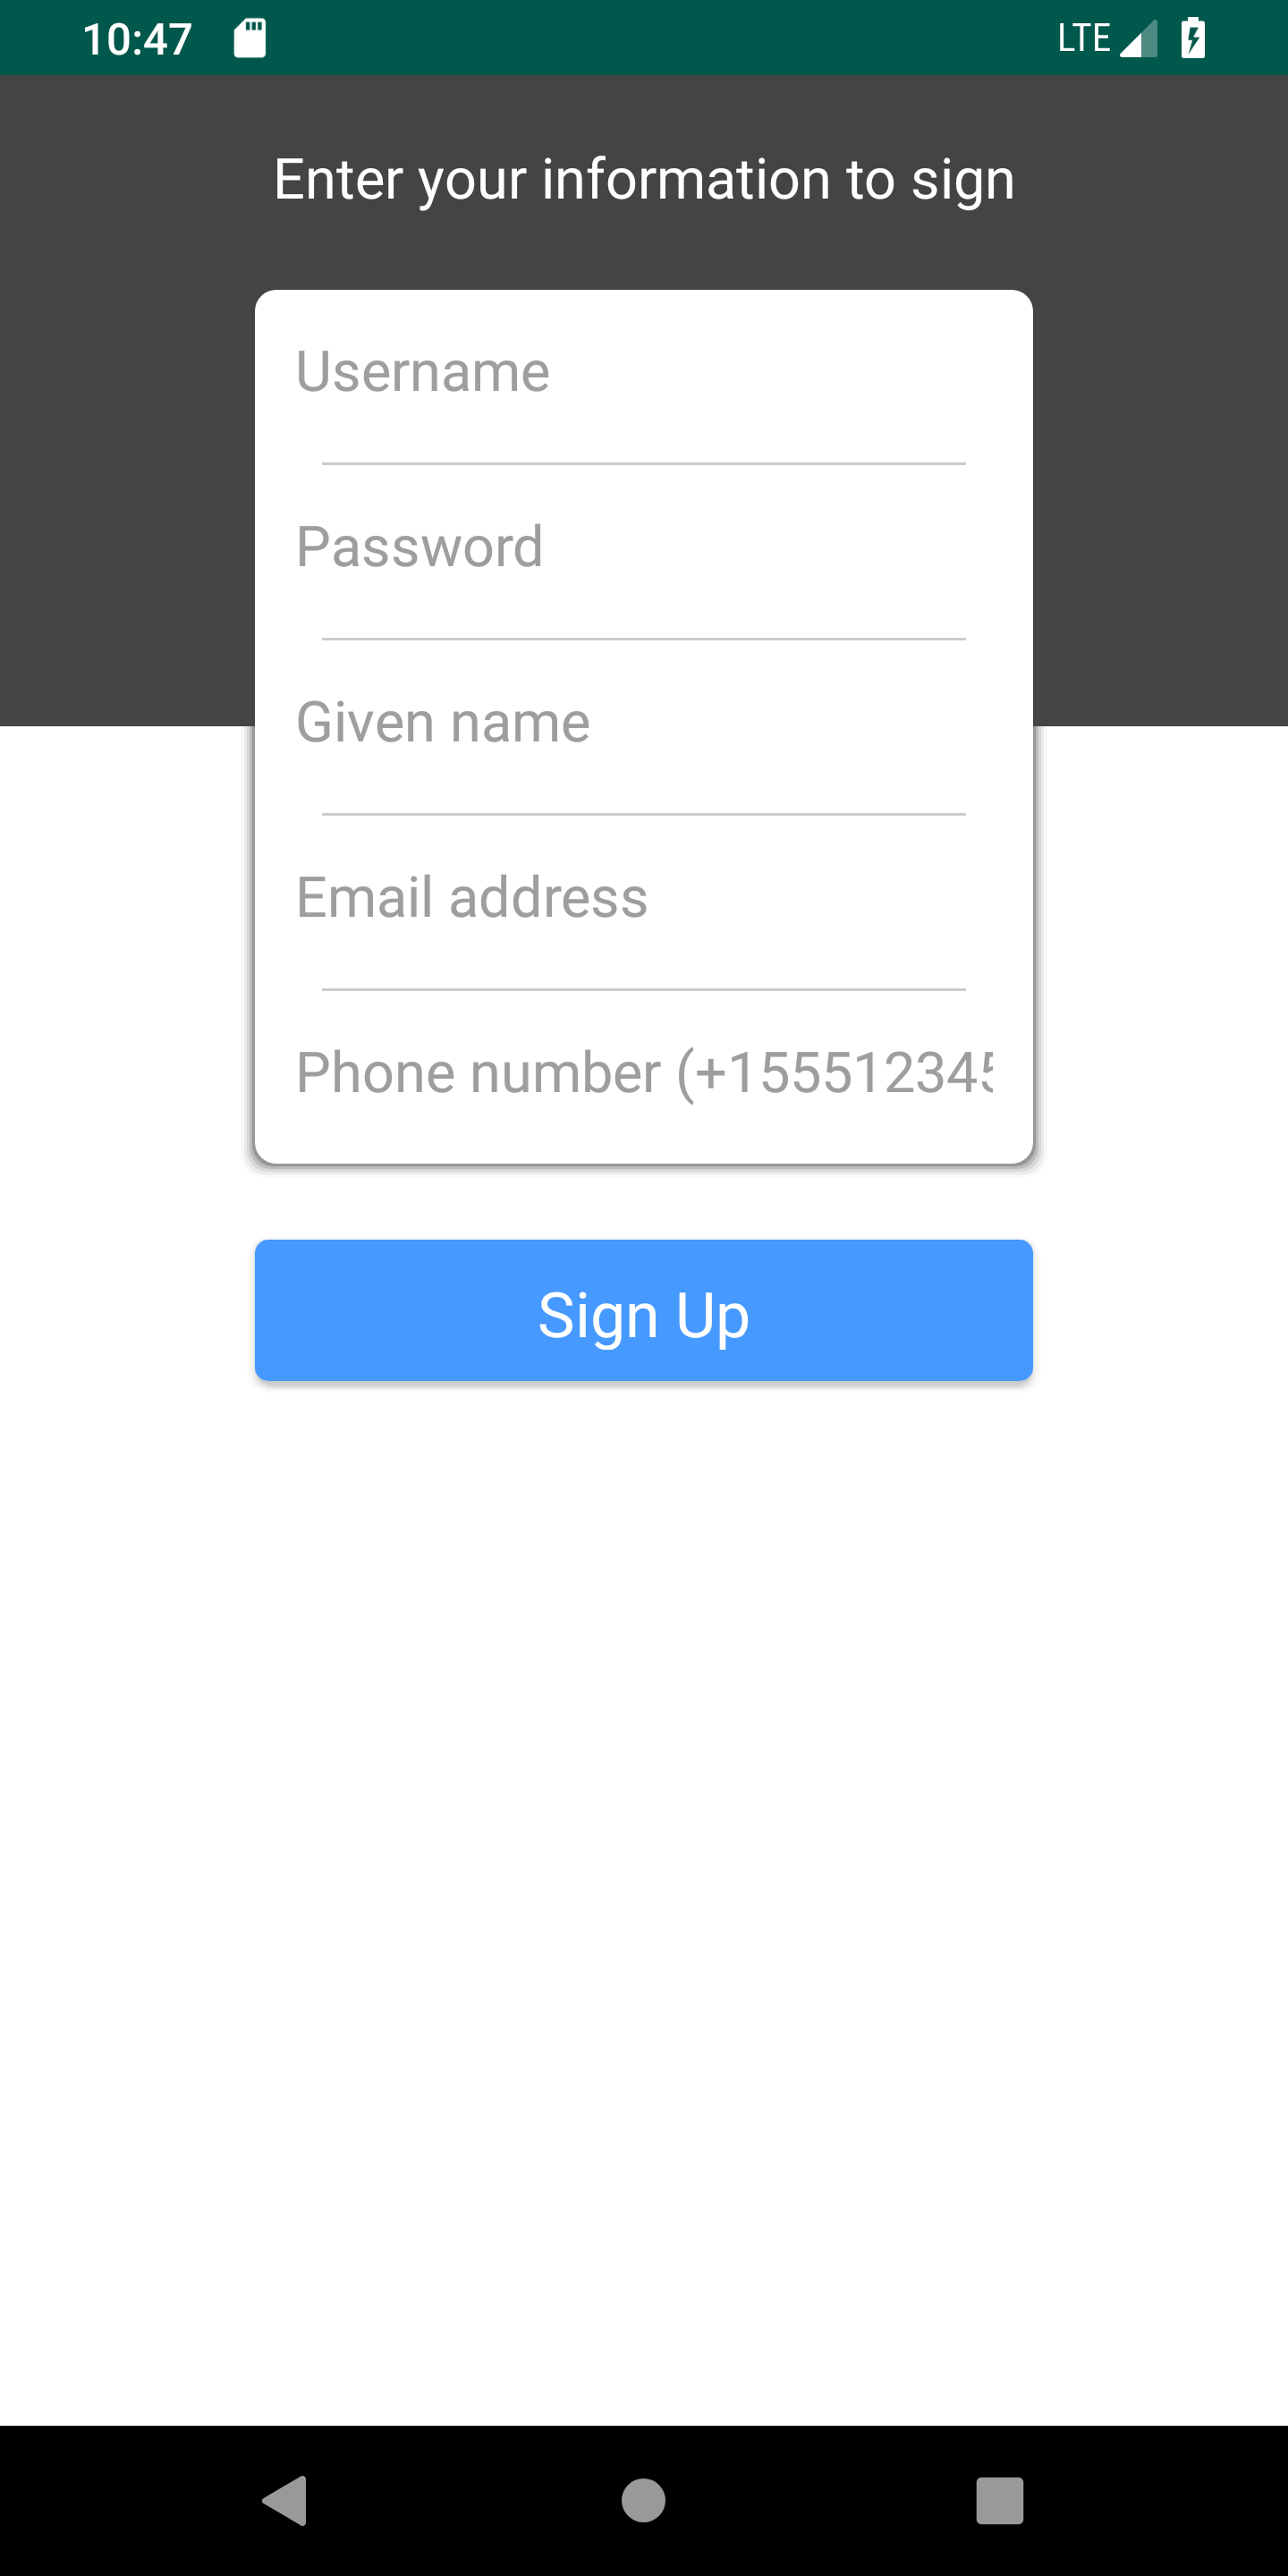
\includegraphics[width=5cm]{../includes/pics/app_registration_form.png}
	\caption{\label{fig:app_registration_form}Form per registrazione utente}
\end{figure}
La procedura di registrazione prevede l'inserimento di varie informazioni:
\begin{itemize}
	\item Username;
	\item Password: di lunghezza uguale o superiore agli 8 caratteri;
	\item Nome (opzionale);
	\item Indirizzo email;
	\item Numero di telefono (opzionale).
\end{itemize}
Una volta inserire le informazioni richieste è necessario cliccare sul pulsante "\textit{Sign Up}". Se i dati sono conformi allora la registrazione avviene correttamente e si riceve una email all'indirizzo specificato per confermare la creazione dell'account; altrimenti verranno segnalati i campi dove sono presenti gli errori.
\subsubsection{Login}
\label{sec:funzionalita_applicazione_login}
L'utente che possiede già l'account può accedere alla sua area personale. 
\begin{figure}[H]
	\centering
	%	\vspace*{-8cm}
	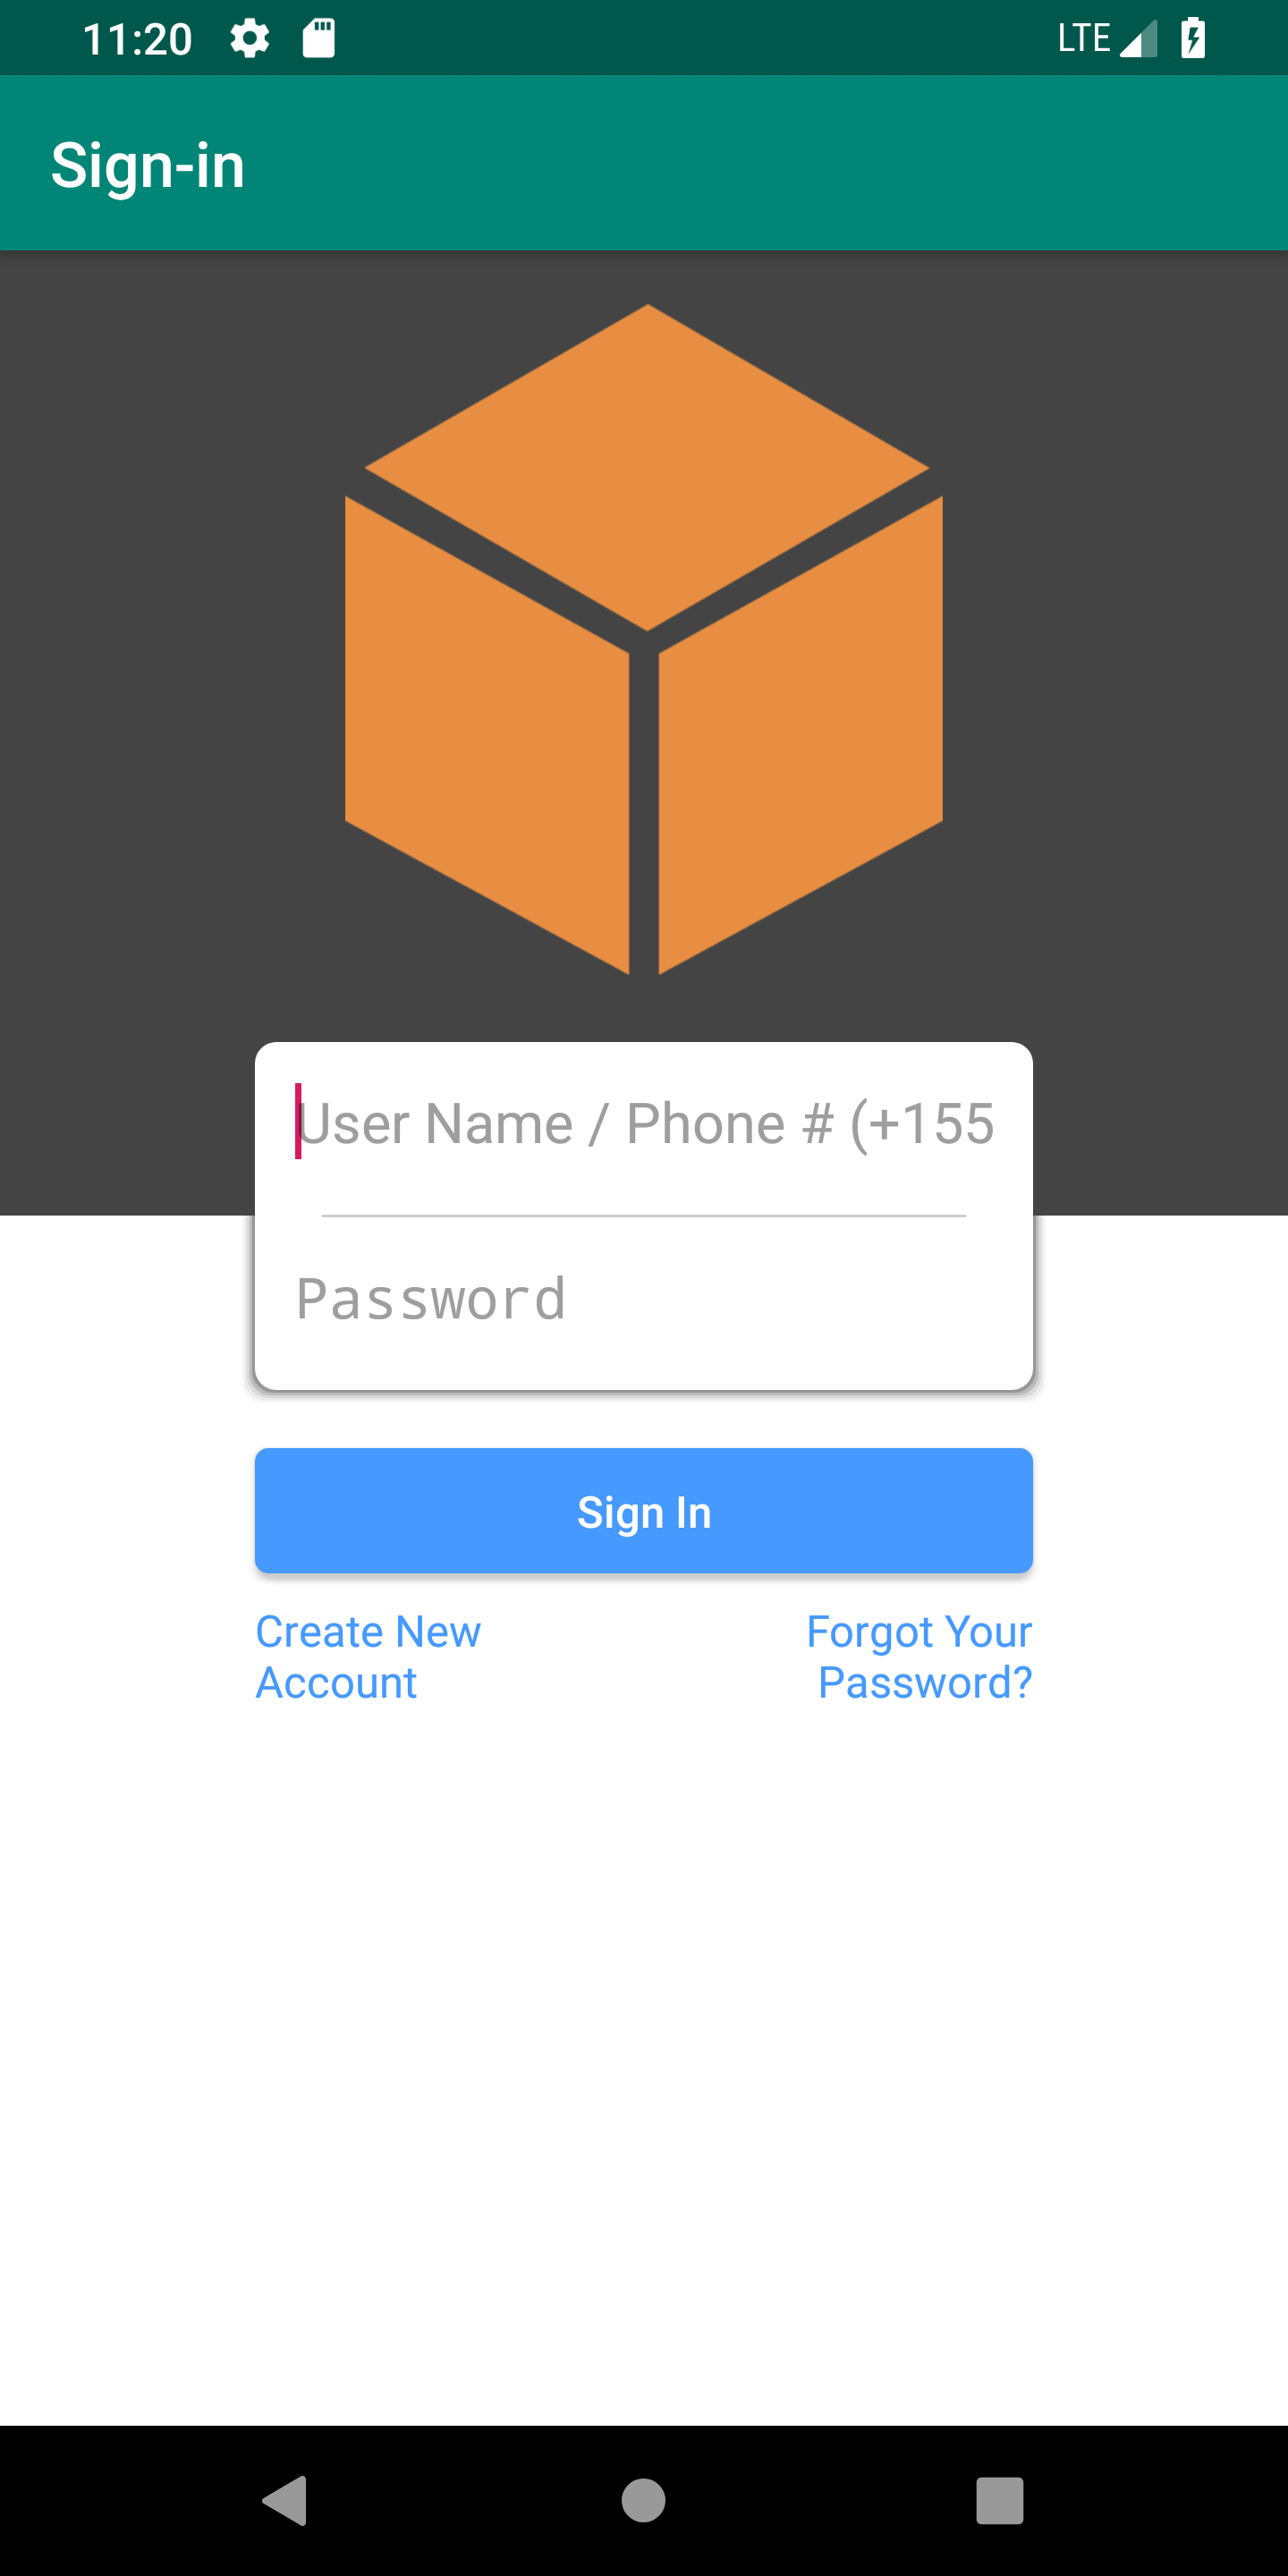
\includegraphics[width=5cm]{../includes/pics/app_login_form.png}
	\caption{\label{fig:app_login_form}Form per login utente}
\end{figure}
La procedura di login prevede l'inserimento delle seguenti informazioni:
\begin{itemize}
	\item Username oppure numero di telefono;
	\item Password.
\end{itemize}
Una volta inserire le informazioni richieste è necessario cliccare sul pulsante 'Sign In'. Se i dati sono conformi allora il login avviene correttamente; altrimenti verranno segnalati i campi dove sono presenti gli errori. 
\subsection{Area personale dell'utente}
\label{sec:sec_area_personale_utente}
Di seguito sono elencate le funzionalità offerte dall'applicazione per gli utenti autenticati.
\subsubsection{Gestione workflow}
All'interno dell'area personale dell'utente è possibile visualizzare tutti i workflow creati dall'utente.
\begin{figure}[H]
	\centering
	%	\vspace*{-8cm}
	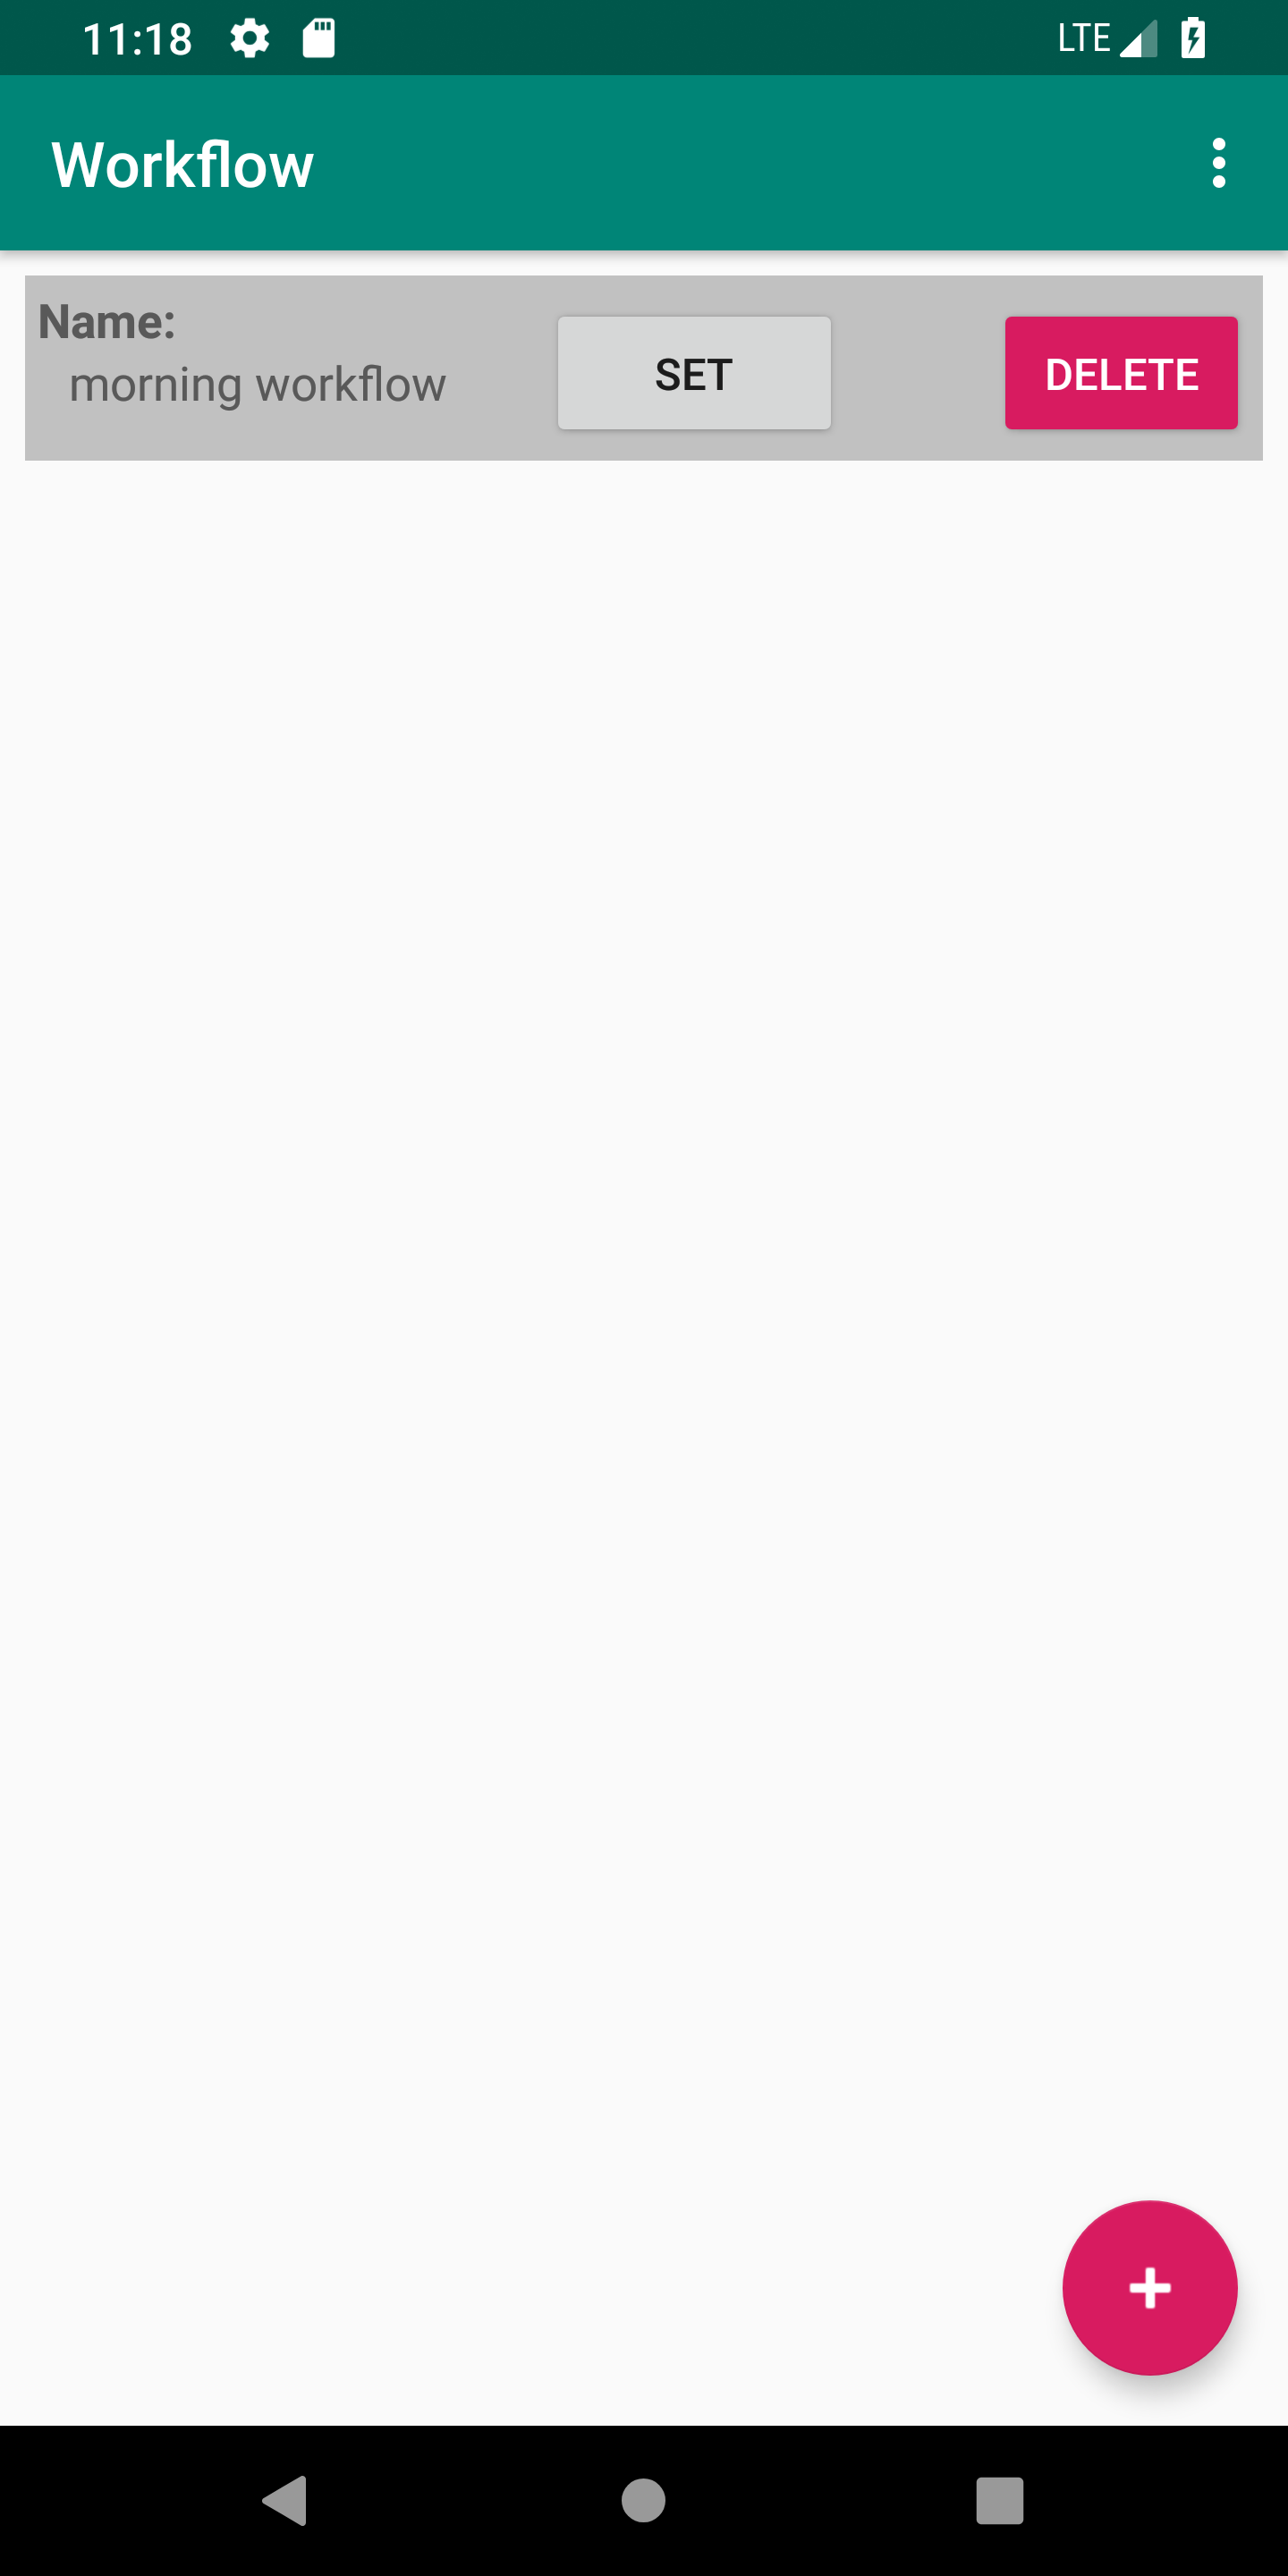
\includegraphics[width=5cm]{../includes/pics/area_workflow_utente.png}
	\caption{\label{fig:area_workflow_utente}Area gestione workflow}
\end{figure}
\pagebreak
\paragraph{Aggiunta nuovo workflow}
\label{sec:sec_aggiunta_nuovo_workflow}
Per creare un nuovo workflow è sufficiente cliccare sul pulsante col segno "+" visualizzato nell'angolo destro inferiore.
Una volta cliccato sul pulsante "+" si apre una nuova schermata rappresentata di seguito.
\begin{figure}[H]
	\centering
	%	\vspace*{-8cm}
	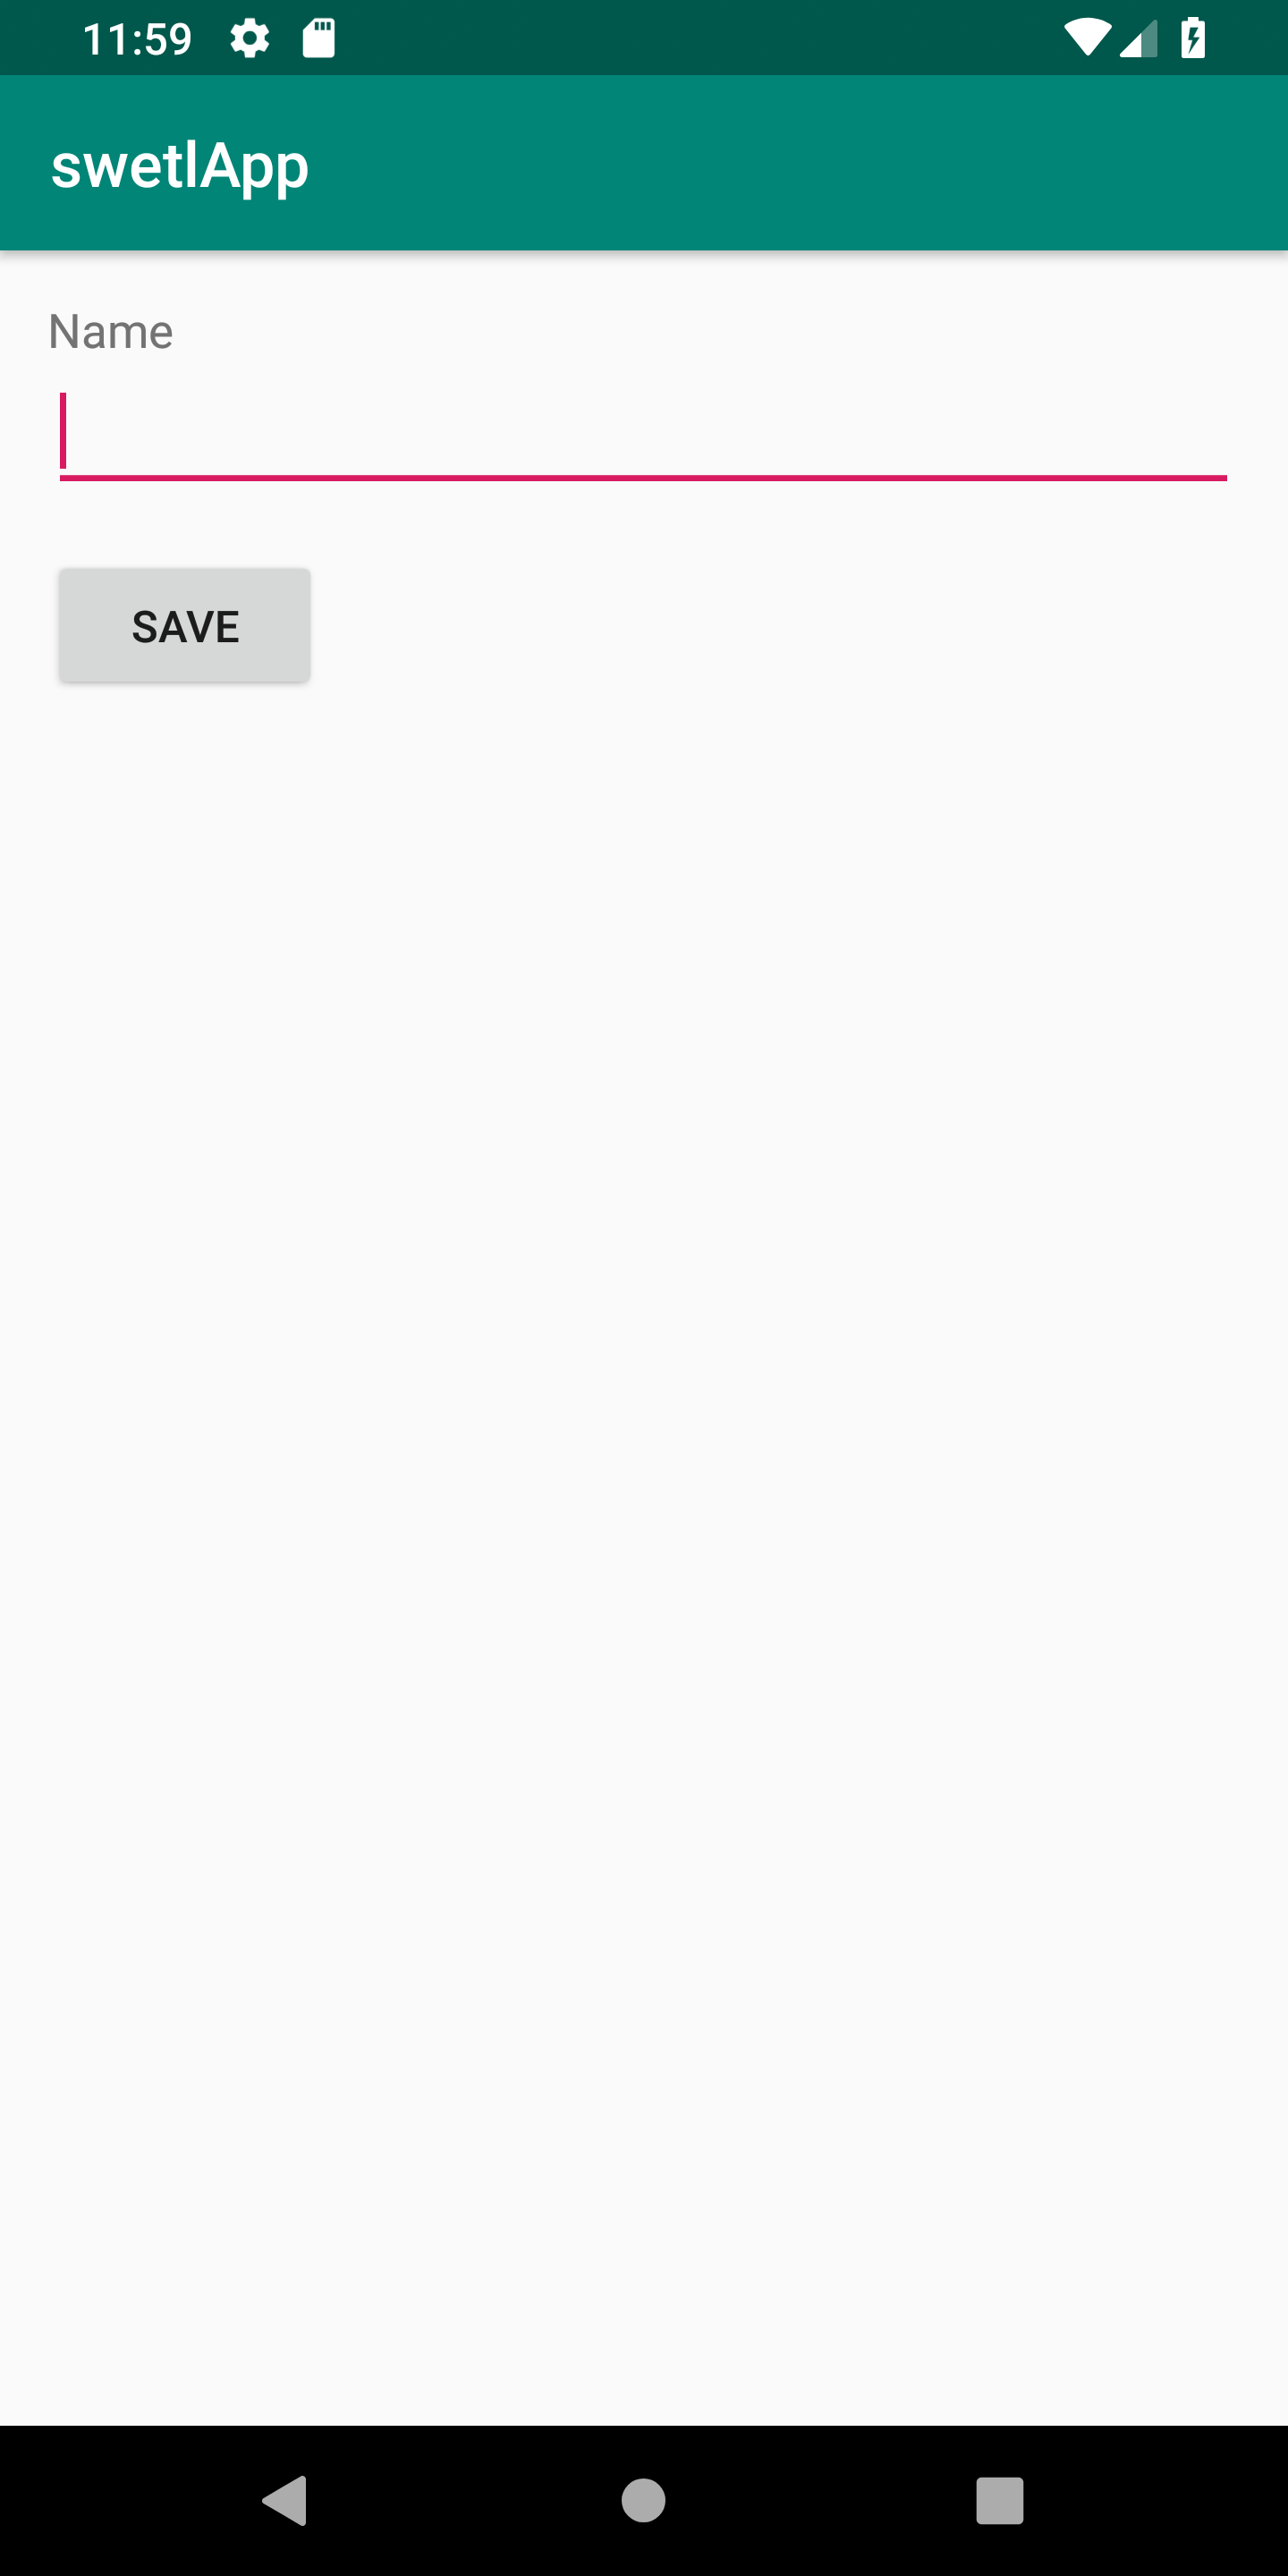
\includegraphics[width=5cm]{../includes/pics/add_workflow.png}
	\caption{\label{fig:add_workflow}Schermata per aggiunta workflow}
\end{figure}
Una volta inserito il nome per il nuovo workflow è necessario cliccare sul pulsante "Save" per confermare la creazione del workflow. Una volta che il workflow viene creato, viene visualizzato nella lista dei workflow creati dall'utente.
\pagebreak
\paragraph{Impostazioni workflow}
\label{sec:sec_impostazioni_workflow}
Per modificare la configurazione di un workflow è necessario cliccare sul pulsante "Set" visualizzato a fianco del nome del workflow.
\begin{figure}[H]
	\centering
	%	\vspace*{-8cm}
	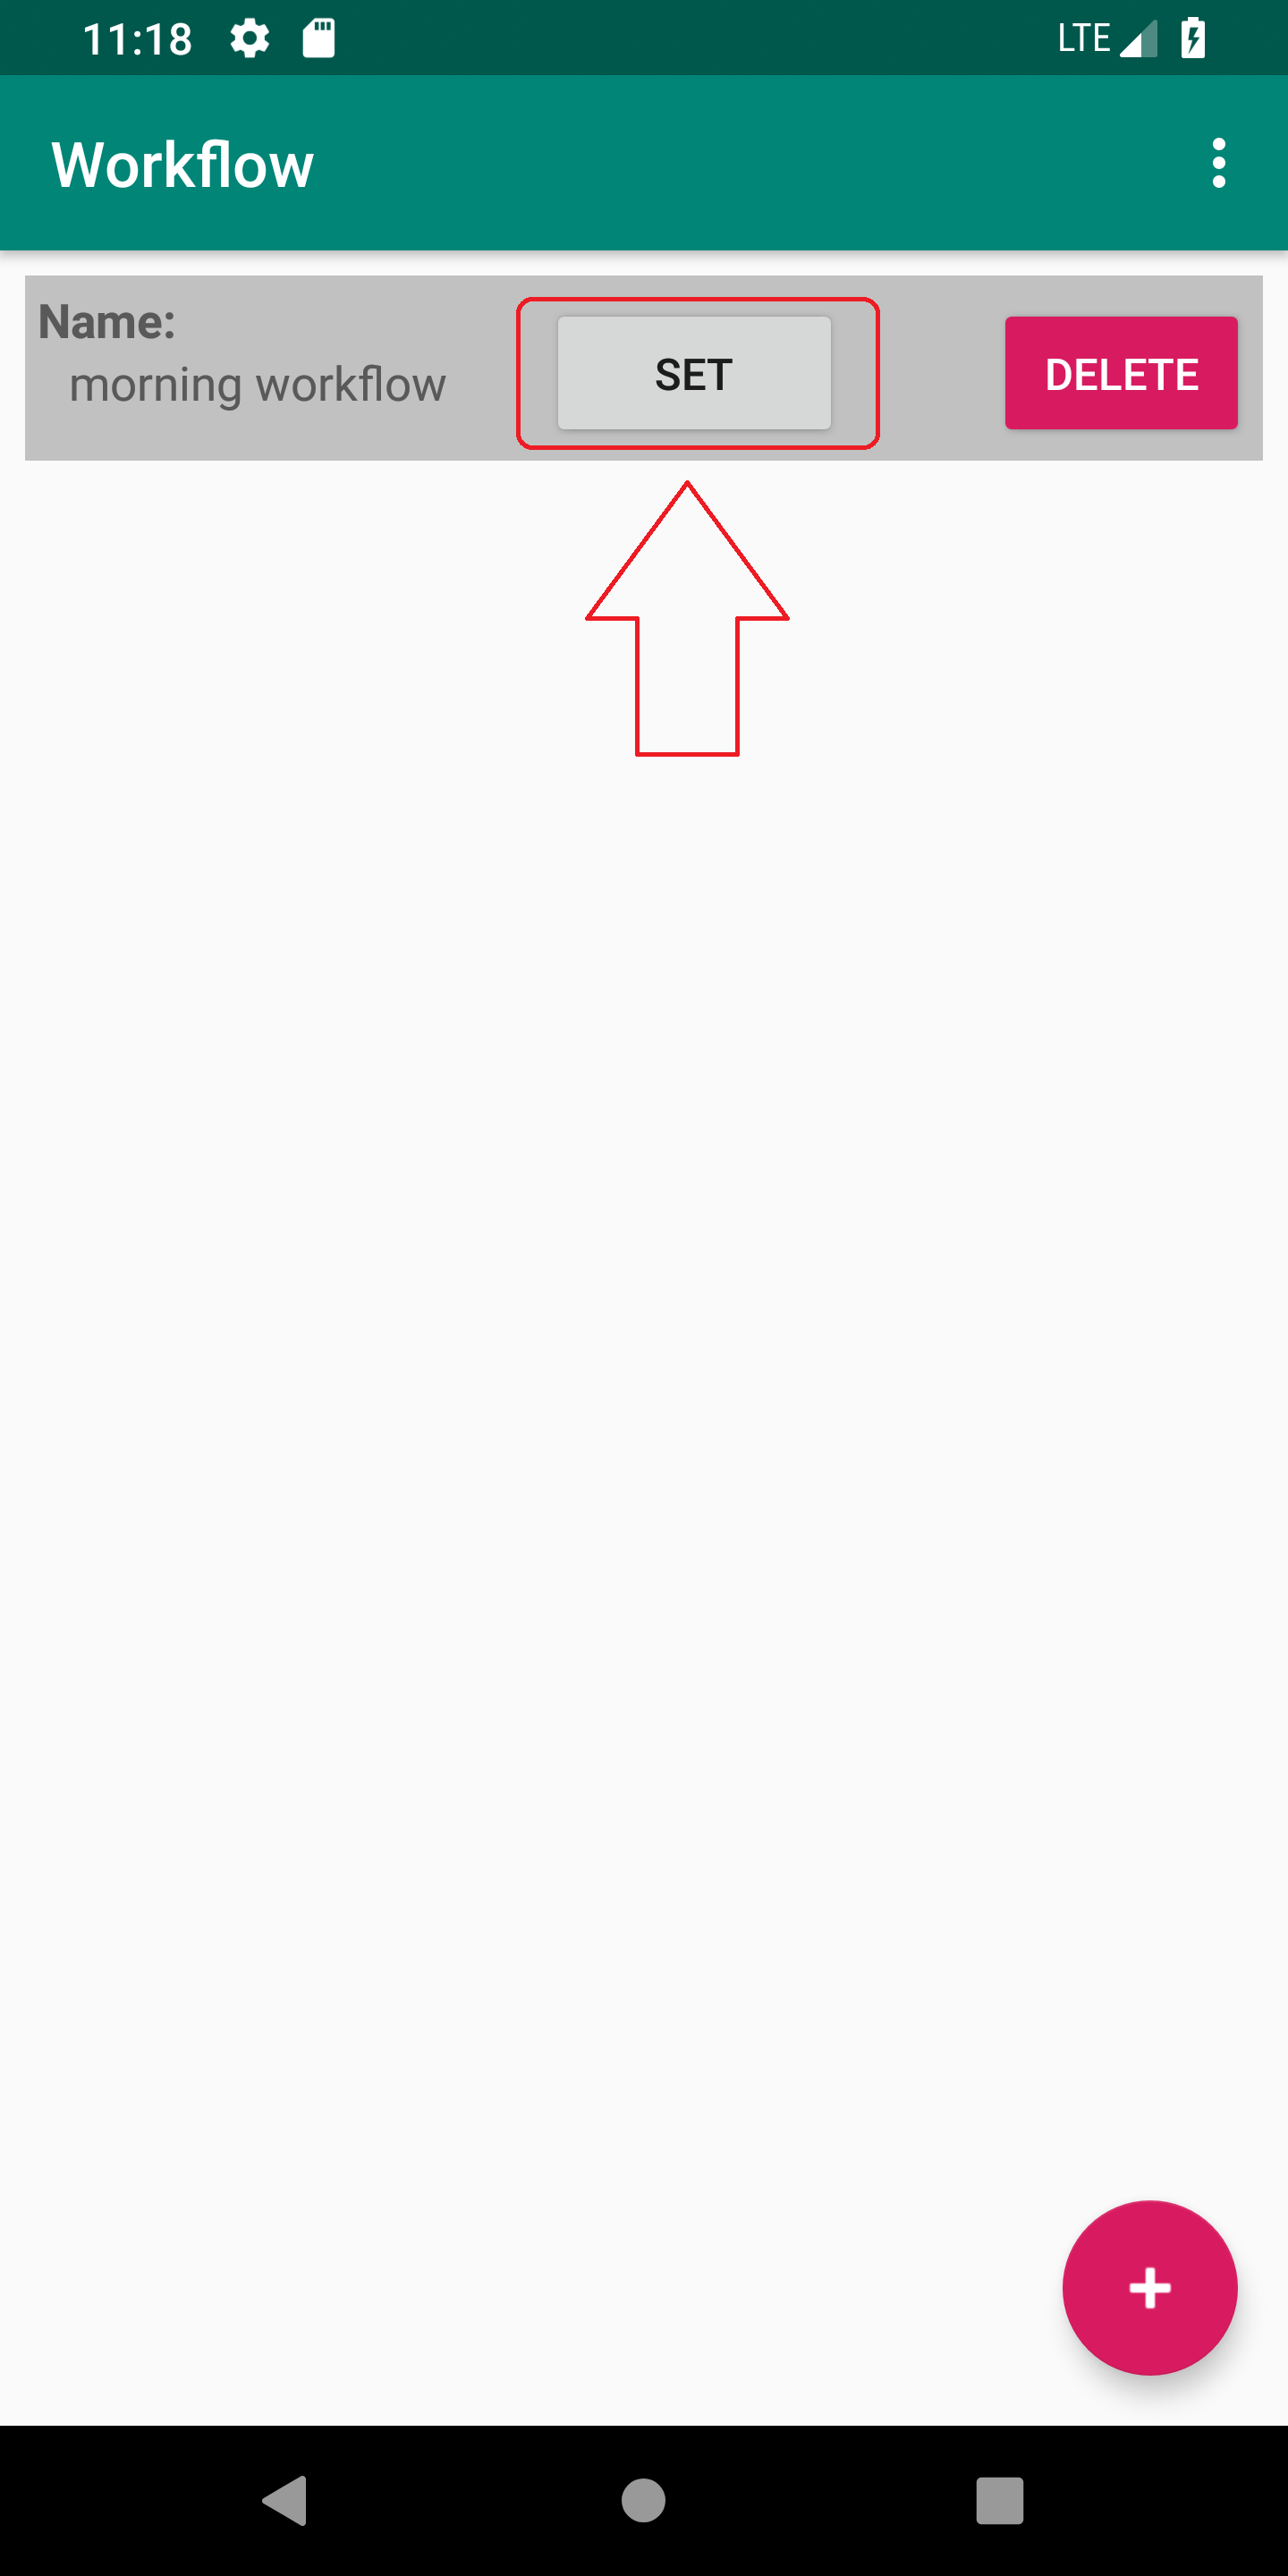
\includegraphics[width=5cm]{../includes/pics/set_button_workflow.png}
	\caption{\label{fig:set_button_workflow}Pulsante per modificare un workflow}
\end{figure}
\pagebreak
Una volta cliccato sul pulsante "Set" si apre una schermata che permette di vedere le micro-azioni (connettori) che compongono il workflow.
\begin{figure}[H]
	\centering
	%	\vspace*{-8cm}
	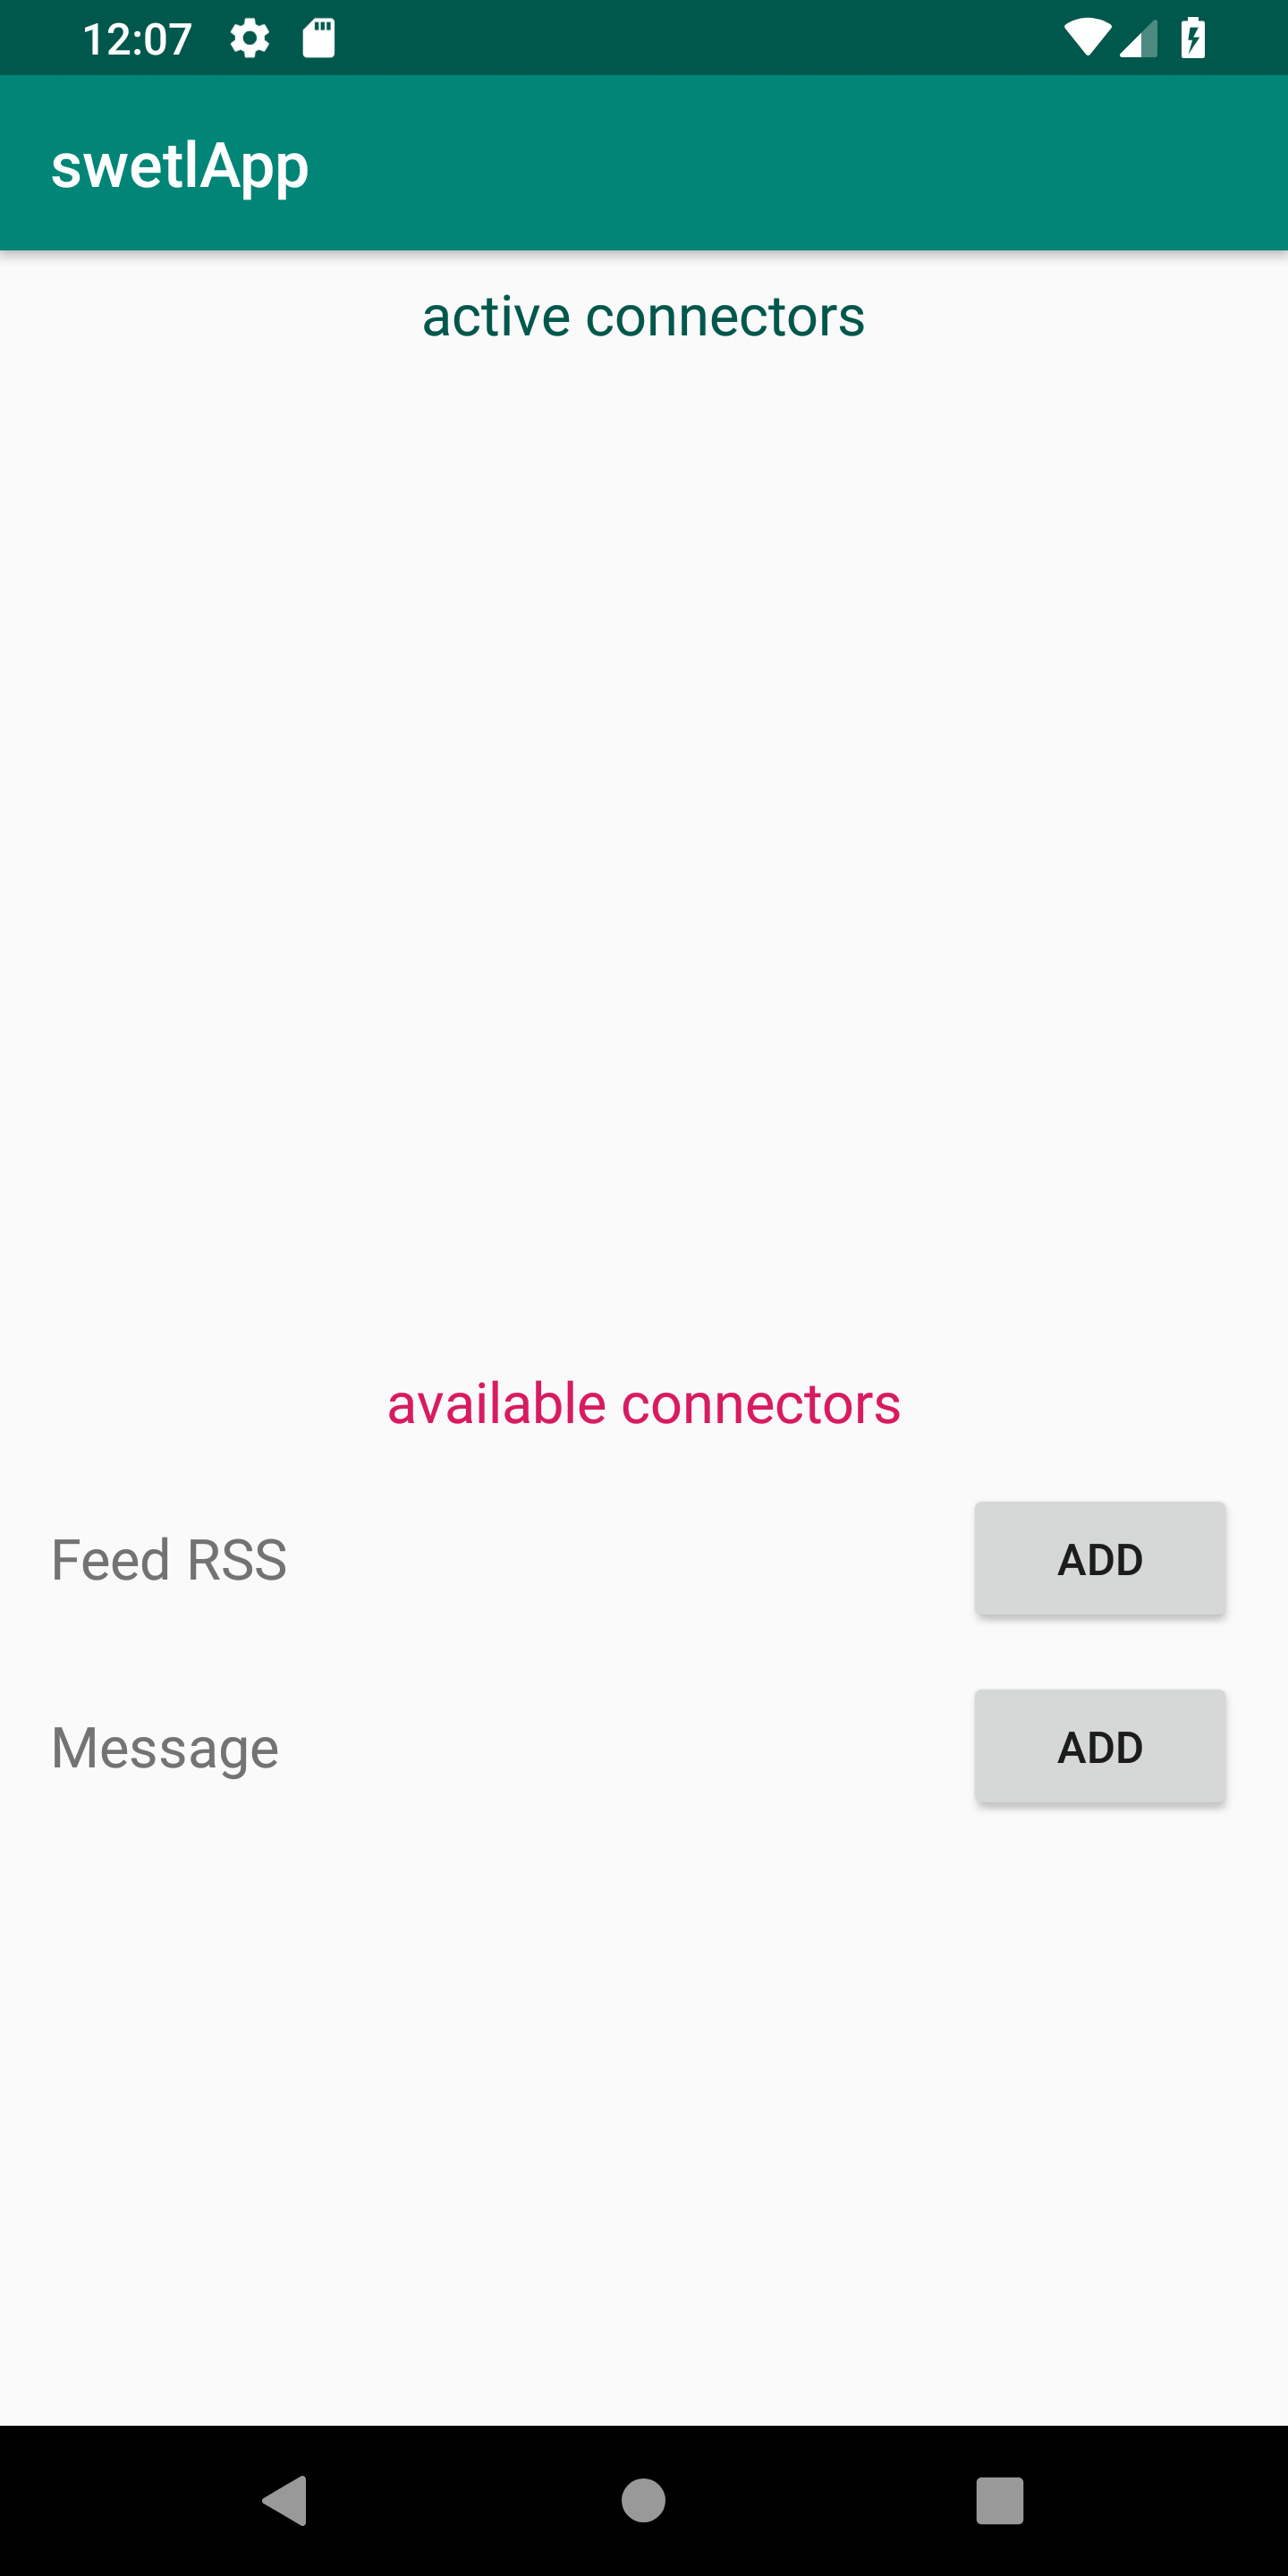
\includegraphics[width=5cm]{../includes/pics/edit_workflow.png}
	\caption{\label{fig:edit_workflow}Pulsante per modificare un workflow}
\end{figure}
Una volta aggiunti i connettori desiderati disponibili sotto la sezione "available connectors" (cliccando sul relativo pulsante "Add") i vari connettori vengono correttamente aggiunti all'interno del workflow soggetto a modifica (sotto la sezione "active connectors").
\begin{figure}[H]
	\centering
	%	\vspace*{-8cm}
	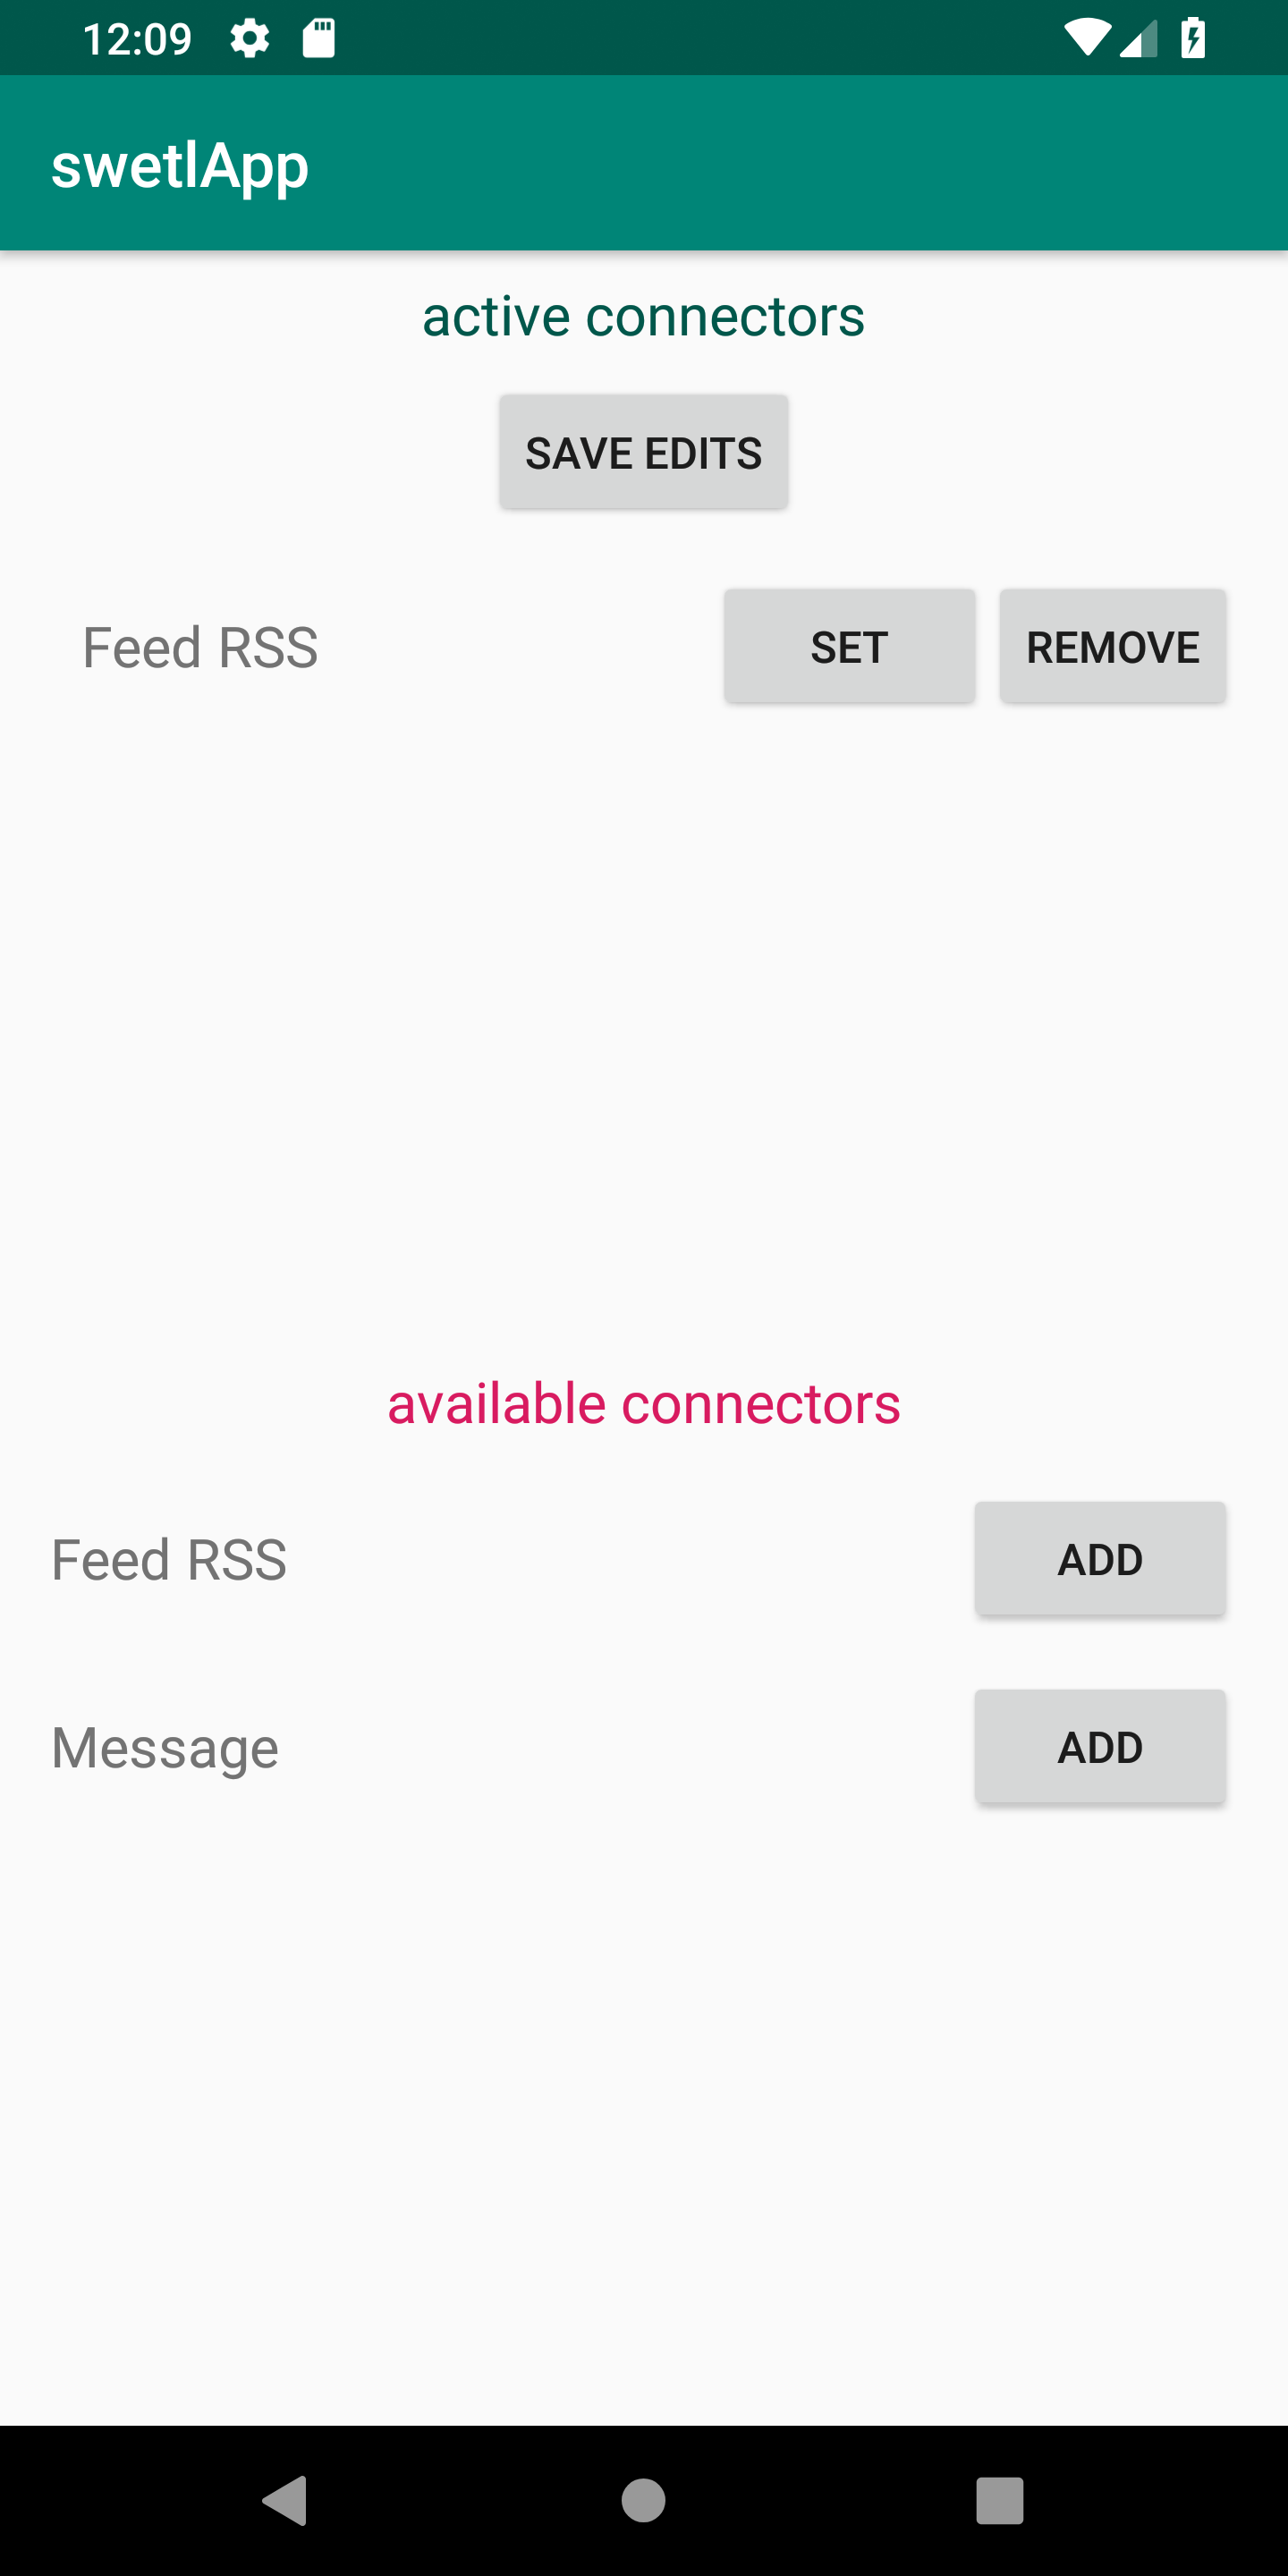
\includegraphics[width=5cm]{../includes/pics/example_connector_added_to_workflow.png}
	\caption{\label{fig:example_connector_added_to_workflow}Visualizzazione connettori aggiunti}
\end{figure}
Per modificare la configurazione del singolo connettore è necessario prmere il pulsante "Set" posto a fianco del nome del connettore, si aprirà una activity da cui sarà possibile impostare i parametri propri del connettore.
Per eliminare il conettore dal workflow corrente è necessario premere il bottone "Remove" posto di fianco al bottone "Set".
Le modifiche eseguite fino ad ora sono solo locali, per renderle effettive è necessario cliccare sul pulsante posto in alto con la scritta "Save edits".
\paragraph{Rimozione workflow}
\label{sec:sec_rimozione_workflow}
Per rimuovere un workflow presente nella propria area personale, è sufficiente cliccare sul pulsante "REMOVE" relativo al workflow da eliminare.